\chapter{Analysis \& Design}\label{chap:design}\label{chap:analysis}
In our problem statement in \Cref{sec:researchstatement}, 
we asked what we can do with wearables in a smart home setting.
In the sections before that, 
we described some of the ways of controlling a smart home. 
One of these was using gestures to control devices in the home. 
As the most used sensor in wearables is the accelerometer (see \Cref{fig:wearables-sensors}), 
it makes sense to utilize this sensor to perform the gestures used to control the devices. 
Our approach to our problem statement is thus using a wearable, 
and its sensors, to perform gestures and thereby control a smart home. 

The goal of our project is to create a system, 
that allows gesture-based communication between the user and smart devices.
We describe the context and the target group of this system in \Cref{sec:environment}.
We want to design the system so that a user, wearing a \emph{wrist wearable}, 
can simply point at a smart device and perform a gesture to control this device. 
This is much like the solution that Reemo (see \Cref{sec:smarthomecontrol}) uses. 
However, we feel that the line-of-sight requirement is a big loss of control, 
as it severely limits the control of objects.
With a line-of-sight requirement, 
it is impossible to control objects in other rooms, 
such as turning on your coffee machine while you are in your bedroom. 
We want to remove this limitation in our solution. 

For this to work, we need a way to determine when a gesture is being performed, 
and which device should perform the action. 
The architecture of the system is presented in \Cref{sec:architecture}.
Gesture recognition is a large subject and will be described in \Cref{sec:gesturerecognition}. 
Furthermore, to determine which device should perform the action, 
without a line of sight requirement, 
we need to know the \emph{indoor location} of the user, 
the position of the device(s) and the heading of the user's gesture. 
We will discuss how we get the location of the devices and the user in \Cref{sec:designindoorlocation}.
At last, as described in \Cref{sec:smarthomes}, 
we need a smart hub to allow communication between the different devices, 
including the wearable, to be able to perform actions on the devices. 
We design a server to hold information about the locations of devices,
and to communicate with a smart hub in \Cref{sec:serverdesign}. 

Our approach to a solution thus requires accurate indoor location, 
a wrist-worn wearable that can recognize gestures, 
and a hub for interoperability between the wearable and the smart devices. 

\section{Environment \& Target Group}\label{sec:environment}

The solution of controlling smart devices with a wearable device could be applicable in a variety of environments including but not limited to: Hospitals, warehouses and homes.
Each of these environments poses a different set of challenges and requirements to the solution, for example a home environment would be a more confined space compared to a warehouse and as such the precision of the solution becomes a more important factor.

We decided to focus on smart homes as we feel that it would result in a system that is more relatable to people, and to us.

\subsection{Target Group}
Our proposed system can have various users but since we have focused on smart home environments, 
our target group would be users thereof. 
We argue that this group will be our main target group, 
as it is most likely to be used by these people for convenience of controlling their smart homes. 
People in this group will currently only be early adopters of technology, 
as the technology (smart homes/devices and wearables) has not yet become common in households.
Based on the trend of IoT, we think that this will no longer be the case in the near future (5-10 years). 

It will also be able to help handicapped people. 
If someone is unable to walk, 
giving that person an easy way to control devices (that may even be out of reach) from afar, 
could provide a better life situation. 
In the same context, by using audio and/or vibrational feedback, 
the system could give blind people a way to determine what he or she is pointing at. 

\section{Architecture}\label{sec:architecture}
The system consists of three layers as illustrated in \Cref{fig:architecture}. 
Each layer can communicate with the layer below and above it if they exist.

The first layer consist of the wearable device and the smartphone. 
The two may be tightly coupled as some wearable watches, 
for example the Apple Watch, relies heavily on the phone. 
The two devices are responsible for listening to new movement data from the wearable, 
\eg new data from the accelerometer and the magnetometer.
The movement data is used for recognizing gestures, 
and the magnetometer data is used for determining direction, 
such that we are able to determine what devices are being pointed at. 
The topmost layer is also responsible for communicating with the beacons, 
in order to retrieve the position of the user, 
and possibly the position of the devices the user can control. 

The topmost layer communicates with a central server developed specifically for this project. 
The server is responsible for storing positions of the smart devices, 
as well as receiving actions, based on interpreted gestures, from the wearable device.
Whenever the wearable device recognizes a gesture, 
the wearable devices sends an action and a device ID to the server.
The server then relays this request to a smart hub. 

The smart hub is responsible for managing the devices that can be controlled using gestures. 
The smart execute the request received from the server, 
on the appropriate smart device. 

When utilizing a smart hub, users must install a hub in their home. 
The hub communicates with the users devices, \eg bulbs, locks and thermostats. 
For privacy reasons, it may be interesting to move the logic of the server to the smart hubs in the users home. 
This would also remove a layer in the architecture, simplifying it.

\begin{figure}[H]
  \centering
  \begin{tikzpicture}
    \node[anchor=center] at (-0.8,0.5) {(1)};
    \node[anchor=center] at (-0.8,-1.5) {(2)};
    \node[anchor=center] at (-0.8,-4) {(3)};
    
    \node[anchor=center] at (2.5,0.5) {Wearable Device};
    \node[anchor=center] at (7.5,0.5) {Mobile Device};
    \draw[thick] (0,0) rectangle (10,1);
    \draw[thick, dashed] (5,0) -- (5,1);
    \draw[thick,->] (10.85,0.5) -- (10.15,0.5);
    \draw[thick] (11,0) rectangle (13,1) node[pos=.5] {Beacons};
    
    \draw[thick] (0,-1) rectangle (10,-2) node[pos=.5] {Server};
    \draw[thick,<->] (5,-0.15) -- (5,-0.85);
    
    \node[anchor=center] at (1.2,-3.4) {SmartThings};
    \draw[thick] (0,-3) rectangle (10,-5);
    \draw[thick,<->] (5,-2.15) -- (5,-2.85);
    \draw[thick] (0.2,-3.8) rectangle (2.7,-4.8) node[pos=.5] (bulb) {Bulb};
    \draw[thick] (2.9,-3.8) rectangle (5.4,-4.8) node[pos=.5] (lock) {Lock};
    \draw[thick] (7.3,-3.8) rectangle (9.8,-4.8) node[pos=.5] (door) {Thermostat};
    \node at ($(lock)!.5!(door)$) {\ldots};
\end{tikzpicture}
  \caption{Architecture of the system.}
  \label{fig:architecture}
\end{figure}

The following components are involved in the architecture:
\begin{description}
    \item[Werable Device] Recognizes gestures and ensures actions are sent. Not included in the implemented prototypes; gesture recognition is performed on a smartphone in out implementation. For more information on gesture recognition, see \Cref{sec:gesturerecognition}.
    \item[Smartphone] Responsible for performing indoor positioning using the beacons. Possibly serves as a medium of communication between the wearable and the server, as some wearable devices require a coupled smartphone.
    \item[Beacons] Utilized for indoor positioning. For more information on this see \Cref{sec:designindoorlocation}.
    \item[Server] A medium of communication between layer (1) and layer (3). For more information about the server, see \Cref{sec:serverdesign}.
    \item[Smart Hub] The hub responsible for communicating with the smart devices. For more information on the smart hub, see \Cref{sec:designsmarthub}.
\end{description}

In the architecture presented in \Cref{fig:architecture}, 
the server is separated from the smart hub. 
In the current prototype, 
the components are physically separated. 
In practice it makes sense to bundle the two components together, 
and keep a virtual separation. 
Based on the current solution, 
the user must install both a server and a smart hub in his home. 
Bundling the two together eases the installation, 
as only a single component will need to be installed, 
and configured by the user.

One way of bundling the two components, 
is to extend the smart hub with the capabilities of the server. 
This is possible if the smart hub solution is open sourced, 
and we have access to the entire implementation. 
Such solution is not possible with other hubs, such as SmartThings.
In order to bundle with such smart hubs, 
the capabilities of our server must be implemented by the company making the smart hub. 


%%% Local Variables:
%%% mode: latex
%%% TeX-master: "../../master"
%%% End:

\section{Gesture Recognition}\label{sec:gesturerecognition}
\section{Indoor Location}\label{sec:designindoorlocation}
In this project, a solution for pointing at a controllable device, \eg a lamp, is proposed. 
In order to determine which device the user points at, 
and thereby intends to control, 
it is necessary to determine the locations of the devices in the system, 
relative to the user. 
We must thus know the location of the user, 
and his controllable devices along with the orientation of the user.

The orientation of the user can be retrieved from any device possessing a magnetometer. 
We found that 49 devices in Vandrico's database contain the magnetometer component. 
Given the orientation of the user, his location and the location of a controllable device, 
we can calculate if the user is looking at, 
or in the direction of, the controllable device. 
We also need to define a visibility range, 
\ie a range (in degrees) such that if the user's direction is \var{directions}, 
then the visibility range \var{range} is $\var{range} = \var{directions} \pm \var{degrees}$, 
where \var{degrees} is a variable defining the size of the visibility range. 
\Cref{fig:visibilityangle} illustrates this. 
In this figure, the user's orientation is \var{o1}, 
and there is two device with orientations \var{o2} and \var{o3}. 
An orientation in degrees is between \num{0} and \num{360}. 
To find if a device with orientation \var{o2} is within the visibility range, 
it is a simple matter of calculating whether $\var{o1} \pm \var{degree}$ is smaller or larger than \var{o2}.

\begin{figure}[!htb]
    \centering
    \def\svgwidth{0.6\textwidth}
    \import{drawings/}{drawings/visibilityangle.pdf_tex}
    \caption{Finding objects in the visibility range. Device 1 is within the range, but Device 2 is not.}
    \label{fig:visibilityangle}
\end{figure}

The focus of this project is not to position devices, 
and as such it was not the intention to spend time developing an entire solution for positioning devices indoors. 
Instead it was desired to find an existing product, 
that could be used to facilitate indoor positioning.
The solution should be available in the early phases of the project, 
in order to start building the system based on the solution for positioning.

As the target group of the project is consumers, 
and not businesses with big budgets, 
it is desired that the price of the technology used for indoor positioning is kept at a minimum. 
This includes the price for any device, 
that may have to be installed on each controllable device in order to position it.

It is assumed that users already own one or more devices that fit within the concept of Internet of Things, 
and are early adapters of such technology. 
However, it easy to imagine that this project can be used in an office environment, 
where employees of varying technological expertise work or in health care. 
Therefore users may have a varying degree of technological expertise, 
and it should be easy to extend the solution with new controllable devices.

Naturally the accuracy of the solution used for indoor positioning plays an important part. 
\Cref{fig:indoor-positioning:incorrect} shows the consequence of an incorrect location. 
If a lamp is estimated to be at another location that it is actually located, 
the user must point to an incorrect location in order to control the lamp.
Furthermore if the estimate is too wide, 
\ie the given area in which the lamp is located is very big, 
there is a greater risk that locations overlap. 
Overlapping locations causes a complexity, 
as it is necessary to determine which device the user desires to control, 
if he points at the overlap as visualized in \Cref{fig:indoor-positioning:overlap}.

\begin{figure}[!htb]
    \centering
    \begin{minipage}[t]{0.45\textwidth}
        \centering
        
\includegraphics[width=0.6\textwidth]{images/incorrect-positioning-estimate.png}
        \caption{Incorrect location estimate. The estimate is visualized as a striped circle.}
        \label{fig:indoor-positioning:incorrect}
    \end{minipage}\qquad
    \begin{minipage}[t]{0.45\textwidth}
        \centering
        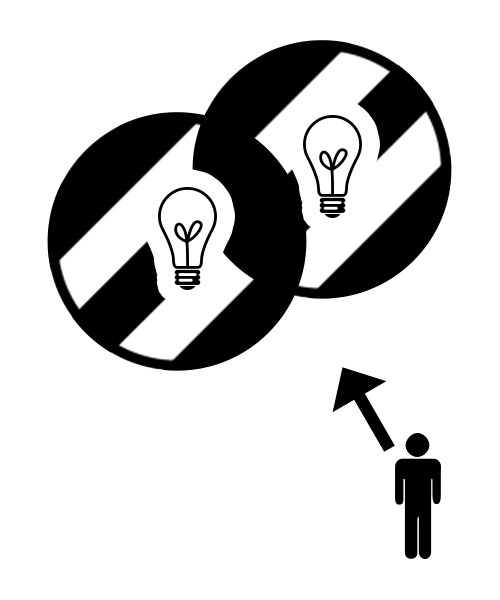
\includegraphics[width=0.6\textwidth]{images/positioning-overlap.png}
        \caption{Overlap of estimated positions. The estimates are visualized as a striped circle.}
        \label{fig:indoor-positioning:overlap}
    \end{minipage}
\end{figure}


\subsection{Analysis of Potential Existing Solution}
This section will be an analysis of commercialized products that offer indoor location.
Only solutions intended for indoor positioning are considered.
GPS is not considered a potential solution as GPS is meant for outdoor positioning, 
and the location offered by GPS tend to have poor accuracy indoors.
We have chosen not to include solutions designed for larger buildings such as airports, malls or warehouses, 
as these does not provide solutions or setups for smaller areas such as rooms or houses. 

\Cref{tbl:indoor-positioning} shows the results of the analysis. 
\begin{table}[!htb]
    \begin{description}[style=multiline,leftmargin=2.5cm]
        \item[Product:] Estimote Beacons and Stickers \cite{estimote}
        \item[Availability:] Beacons and Stickers are shipping. SDKs available.
        \item[Technology:] iBeacon protocol.
        \item[Price:] \SI{99}[\$]{} for beacons. \SI{99}[\$]{} for 10 stickers, one per device to be positioned.
        \item[Ease of use:] Initial installation of beacons. Attach each sticker to device.
        \item[Accuracy:] Unknown. Desired to be less than five meters. \\ \todo[author=Simon]{Update after conducting tests.} 
        
        \item[Product:] Pozyx \cite{pozyx}
        \item[Availability:] Available for preorder.
        \item[Technology:] Ultra-wideband (UWB).
        \item[Price:] \$368 for anchors. \SI{123}[\$]{} for each device to be positioned, plus supported Arduino.
        \item[Ease of use:] Initial installation of anchors. One tag for each device, plus supported Arduino. Not meant for mounting.
        \item[Accuracy:] Claimed to be 10 cm. Untested. \\
        
        \item[Product:] SmartActionSLAM \cite{SASLAM}
        \item[Availability:] Android Application (research). Not commercialized.
        \item[Technology:] Smartphone sensors.
        \item[Price:] N/A.
        \item[Ease of use:] Requires modification of source code (available) to get real-time position. 
        \item[Accuracy:] Reported to have a mean error of 0.34m (only using smartphone and no external sensors).\\
        
        \item[Product:] DecaWave's DW1000 \cite{decawave}
        \item[Availability:] Available in stores. 
        \item[Technology:] Ultra-wideband (UWB)
        \item[Price:] Chips are \SI{12.50}[\$]{}, transceiver module is \SI{25}[\$]{}. Evaluation kits are available for \SI{589}[\$]{} and \SI{990}[\$]{} 
        \item[Ease of use:] No SDK and requires implementing the chips on a board yourself. 
        \item[Accuracy:] Claimed to be 10cm. 
        \end{description}
    \caption{Assessment of potential solutions for indoor positioning. Please note that all prices are converted to U.S. dollars from their respective currency. Prices include the minimum available hardware for positioning a device.}
    \label{tbl:indoor-positioning}
\end{table}

Estimote gives a solution using Bluetooth Low Energy (BLE) beacons using the iBeacon protocol. 
The beacons can be mounted on walls in a room or building, 
and then by using the signal strength of each beacon (an iBeacon feature), 
it can estimate how far away the user is. 
Estimote's solution is available as a consumer product.

Pozyx and DecaWave use a wireless radio technology known as ultra-wideband, which works much like BLE but at a different frequency. 
Like Estimote, it also requires setting up ``anchors'' and then using the signal strength to find the location. 
No easy to use consumer product is availably for either of these.

SmartActionSLAM is an Android application from research done by Hardegger \etal \cite{SASLAM}. 
This solution is a lot different from most other indoor location solutions. 
It \emph{calculates} an estimated location by counting steps and estimating step length and direction. 
In theory it can be adapted to almost any smartphone, 
but requires a lot of work to adapt the released code from the research project. 

\subsection{Estimote}

Beacons are used for indoor location in this project. Estimote is one of many vendors of iBeacons. Common use cases for beacons include monitoring if the user enters a specific region of an area. This can be used to push location specific information or advertisement when a user is near a shop or even a certain product in that shop.

Estimote not only focus on typical use cases for beacons like entering a specific region, but have also specialized in indoor location of users using the beacon technology. The company developed the Estimote Indoor Location application for iOS\footnote{https://itunes.apple.com/us/app/estimote-indoor-location/id963704810} which is meant to ease configuration needed for indoor location. A user will install the beacons in a room by placing one beacon on each wall. Next the user walks along the perimeter of the room and thereby registering the location of the beacons by collecting signal strengths from the beacons and data from the phones accelerometer and/or gyroscope.
After the configuration, the application has estimated the length of and placement of walls allong with the signal strengths of each beacon.

During our tests we found that the approach for configuring the indoor locationing describe above works terribly or not at all. After configurin the room, the application would show an illustration of the registered room and we found the measurements to to be very inaccurate. The Estimote Indoor Location application was therefore abandoned for configuring a room.

\subsubsection{Configuring Rooms Programmatically}

Estimote provides Estimote Indoor Location SDK\footnote{https://github.com/Estimote/iOS-Indoor-SDK} to perform indoor locationing using beacons on iOS. The SDK provides two mechanisms for configuring a room for indoor positioning.

\begin{enumerate}
\item Using the built-in controller. The component presents the user with a guided configuration similar to the one used in the Estimote Indoor Location application.
\item Programmatically using the \texttt{ESTLocationBuilder} class.
\end{enumerate}

The built-in controller was abandoned as it uses the exact same technology as the Estimote Indoor Location application and therefore results in poor accuracy.

The \texttt{ESTLocationBuilder} lets developers configure a room programmatically by passing XY-points and an orientation to the builder. The X and Y value of each point is measured in meters. Therefore a point $(0, 0$) to $(0, 5)$ represents a horisontal line of five meters and the set of points $\{(0,0),(0,5),(5,5),(5,0)\}$ represents a room of size 5 meters by 5 meters.

\begin{listing}
\begin{swiftcode}
        let locationBuilder = ESTLocationBuilder()
        locationBuilder.setLocationBoundaryPoints([
            ESTPoint(x: 0.cmToMeter(), y: 0.cmToMeter()),
            ESTPoint(x: 537.cmToMeter(), y: 0.cmToMeter()),
            ESTPoint(x: 537.cmToMeter(), y: 60.cmToMeter()),
            ESTPoint(x: 690.cmToMeter(), y: 60.cmToMeter()),
            ESTPoint(x: 690.cmToMeter(), y: 385.cmToMeter()),
            ESTPoint(x: 0.cmToMeter(), y: 385.cmToMeter()),
        ])
        
        let ice3 = "dec18deac0c5"
        let blueberry3 = "f13173ad3185"
        let ice2 = "d470d26d33f3"
        let mint3 = "e6d39dee79c9"
        
        locationBuilder.addBeaconIdentifiedByMac(blueberry3, atBoundarySegmentIndex: 0, inDistance: 422.cmToMeter(), fromSide: .RightSide)
        locationBuilder.addBeaconIdentifiedByMac(ice3, atBoundarySegmentIndex: 3, inDistance: 222.cmToMeter(), fromSide: .RightSide)
        locationBuilder.addBeaconIdentifiedByMac(mint3, atBoundarySegmentIndex: 4, inDistance: 335.cmToMeter(), fromSide: .LeftSide)
        locationBuilder.addBeaconIdentifiedByMac(ice2, atBoundarySegmentIndex: 5, inDistance: 165.cmToMeter(), fromSide: .LeftSide)
        locationBuilder.setLocationOrientation(130)
        locationBuilder.setLocationName("Gros Stue")
        
        let location = locationBuilder.build()
\end{swiftcode}
\caption{Example usage of the \texttt{ESTLocationBuilder} class.}
\label{lst:estlocationbuilder}
\end{listing}

Listing \ref{lst:estlocationbuilder} shows how we used the \texttt{ESTLocationBuilder} to create a model of a real world living room. The resulting model is illustrated in figure \ref{fig:estlocationbuilder-livingroom}.

The builder is configured with six points that gives information about the shape of the room. Next, the beacons are added to the walls of the room. Beacons are added with the identifier of the beacon. Lastly the orientation of the room relative to north and the name of the room is set. When the room has been configured it can be stored on the users Estimote account using the Estimote SDK.

Using the \texttt{ESTLocationBuilder} to model a room reduces any uncertainties in estimating the users location caused by an imprecise model of the room.

\begin{figure}
\centering
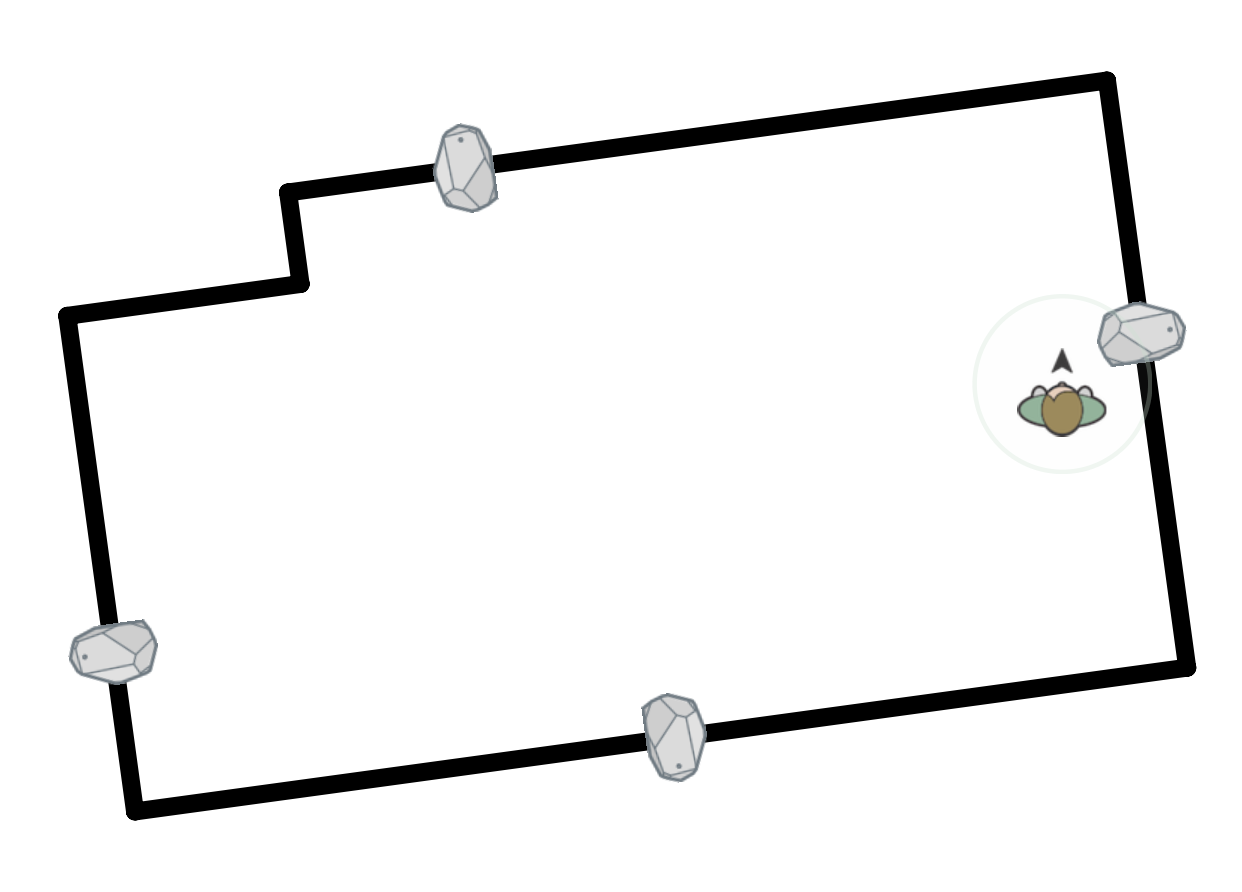
\includegraphics[width=0.33\textwidth]{images/living-room}
\caption{Model created using the \texttt{ESTLocationBuilder} as shown in listing \ref{lst:estlocationbuilder}. Note that the model is rotated accordingly to the orientation of the room and the position of north relative to the user.}
\label{fig:estlocationbuilder-livingroom}
\end{figure}

\subsubsection{Ranging in the Background}

There are two distinct ways of locating a user when using iBeacon \cite{estimote:monitoring-ranging}.

\begin{itemize}
\item Region monitoring is performed to check if a user enters or leaves a specific region. A region is a geofence, a virtual perimeter around some location. Such region could be used to check if a user arrives or leaves his house, his workplace or if he is nearby a shop encapsulated in a geofence. Regions are useful for performing simple home automation, e.g. turn the lights on when the user arrives at home and turn them off when they leave.
\item Ranging is more granular than region monitoring and is used to continuously retrieve the set of beacons in range along with an estimated distance to them based on the signal strengths. Ranging is used to get a granular user position.
\end{itemize}

According to both Apple and Estimote it is preferred that ranging is only performed while the application is in the foreground, that is, the application is on the screen and the user is likely to interact with the application. The reason for this is that ranging for beacons can have a negativ impact on the battery life where as the region monitoring do not use as much battery power.

While Apple and Estimote advise agains performing beacon ranging in the background, it is possible \cite{apple:monitoring-ibeacon} \cite{estimote:monitoring-ranging}.

%%% Local Variables:
%%% mode: latex
%%% TeX-master: "../../master"
%%% TeX-command-extra-options: "-shell-escape"
%%% End:

%%% Local Variables:
%%% mode: latex
%%% TeX-master: "../../master"
%%% TeX-command-extra-options: "-shell-escape"
%%% End:

\section{Server}
The server of our system manages the communication between the user and the devices. 
The user issues a request containing the actions to be executed and on which device. 
The server must also contain information about the smart devices available,
and be able to provide the wearable with this information. 

We want to provide a very simple Representational State Transfer (REST) interface.
The REST interface should provide the following methods:

\begin{enumerate}
  \item \texttt{GET /devices} - Return a list of available devices
  \item \texttt{POST /} with form data [\texttt{action}, \texttt{id}] - Perform \texttt{action} on device with ID \texttt{id}
\end{enumerate}

Each device handled by the server have descriptive information such as \texttt{name}, \texttt{id} and location. 
A class diagram of the \texttt{Device} class can be seen in \Cref{fig:deviceclass}.

\begin{figure}[!htb]
  \centering
  \begin{tikzpicture} 
    \umlclass[x=0,y=0]{Device}{
      +/- id : Int \\
      +/- actions : Set[String] \\
      +/- state : String \\
      + name : String \\
      + coordinates : Tuple(Float, Float)
    }{
    + canPerformAction(action)
    } 
  \end{tikzpicture}
  \label{fig:deviceclass}
  \caption{Class diagram of the \texttt{Device} class.}
\end{figure}

In the diagram, \texttt{actions} describes the set of actions available for that devices, \eg $\{\var{turnOn}, \var{turnOff}\}$. 
The state describes the state of the devices, 
\eg $\var{state} \in \{\var{on}, \var{off}\}$ for devices with only binary states, 
but could also for a lamp, be a number between \num{0} and \num{100} describing the brightness of the light. 
The state should come from the smart hub and/or the device itself. 
The tuple of \texttt{coordinates} describes the location of the smart device. 
The \texttt{canPerformAction(action)} method is used to make sure that we do not try to perform an action on a device that cannot perform that action. 

\subsection{Communication with Smart Hub}
We have chosen to use HomePort (introduced in \Cref{sec:homeport}) as our smart hub in this project.
The reason why we chose to use HomePort is that is it easily available for us, 
since it is a research project from our university. 
This means that we have access to the source code and are able to modify the code to better suit our needs. 
Furthermore, HomePort can control the Phidget devices we have available, 
making it easier and faster to setup than to order a commerciel product, 
or implement support for these devices on the open source solutions described in \Cref{sec:smarthubsmarket}. 

As mentioned in \Cref{sec:homeport}, we can get list of available devices by sending a \texttt{GET} request to \texttt{/devices} on the HomePort server. 
The list is returned as Extensible Markup Language (XML). 
Since we prefer to use JavaScript Object Notation (JSON) format instead of HomePort's XML, 
we need to translate from XML to JSON in the server. 

To execute an action on a device, we can send a \texttt{PUT} request to the HomePort server. 
We use the \texttt{id} of the device to construct the proper HomePort URL. 
However, HomePort uses numerical values for actions (0 = 'off', 1 = 'on'), 
so our server also needs to be able to map the actions to a numerical value in order for HomePort to process it. 



